\documentclass[a4paper]{article} %可加上 twocolumn 來變成雙欄格式
\usepackage{fontspec}   %加這個就可以設定字體
\usepackage{xeCJK}       %讓中英文字體分開設置
\usepackage{indentfirst}
\usepackage{listings}
\usepackage[newfloat]{minted}
\usepackage{float}
\usepackage{graphicx}
\usepackage{caption}
\usepackage{fancyhdr}
\usepackage{hyperref}
\usepackage{amsmath}
\usepackage{multirow}
\usepackage[dvipsnames]{xcolor}
\usepackage{graphicx}
\usepackage{tabularx}
\usepackage{booktabs}
\usepackage{caption}
\usepackage{subcaption}
\usepackage{pifont}
\usepackage{amssymb}
\usepackage[backend=biber]{biblatex}
\addbibresource{main.bib}


\usepackage{pdftexcmds}
\usepackage{catchfile}
\usepackage{ifluatex}
\usepackage{ifplatform}

\usepackage[breakable, listings, skins, minted]{tcolorbox}
\usepackage{etoolbox}
\setminted{fontsize=\footnotesize}
\renewtcblisting{minted}{%
    listing engine=minted,
    minted language=python,
    listing only,
    breakable,
    enhanced,
    minted options = {
        linenos,
        breaklines=true,
        breakbefore=.,
        % fontsize=\footnotesize,
        numbersep=2mm
    },
    overlay={%
        \begin{tcbclipinterior}
            \fill[gray!25] (frame.south west) rectangle ([xshift=4mm]frame.north west);
        \end{tcbclipinterior}
    }
}

\usepackage[
top=1.5cm,
bottom=0.75cm,
left=1.5cm,
right=1.5cm,
includehead,includefoot,
heightrounded, % to avoid spurious underfull messages
]{geometry}

\newenvironment{code}{\captionsetup{type=listing}}{}
\SetupFloatingEnvironment{listing}{name=Code}


% set the title and name
\title{VRDL HW3 Report}
\author{112550011 李佑軒}
\date{\today}


% \setCJKmainfont{Noto Serif TC}
\setCJKmainfont{Microsoft JhengHei}


\ifwindows
\setmonofont[Mapping=tex-text]{Consolas}
\fi

\XeTeXlinebreaklocale "zh"             %這兩行一定要加，中文才能自動換行
\XeTeXlinebreakskip = 0pt plus 1pt     %這兩行一定要加，中文才能自動換行

\newcommand*{\dif}{\mathop{}\!\mathrm{d}}

\begin{document}
\maketitle % write the title, name and date

\section{Introduction}

{\sloppy Github link: \url{https://github.com/Yu-Hsuan-1220/NYCU_Visual_Recognition_Using_Deep_Learning/tree/main/HW3}\par}

The objective of this assignment is to develop a high-performance instance segmentation system for medical cell microscopy images, capable of detecting and segmenting individual cell instances across four distinct categories. The primary evaluation metric is $\text{mAP}@50$ for segmentation masks, which demands both accurate object localization and precise pixel-level mask prediction.

The dataset consists of TIFF microscopy images where each image can contain many of densely packed cell instances with significant variation in size, shape, and scale. The key challenges are: (1) segmenting tightly overlapping cells across vastly different scales, and (2) generalizing robustly from limited training data.

Our approach adopts \textbf{Cascade Mask R-CNN} with a \textbf{ConvNeXt-V2-Base} backbone and \textbf{Feature Pyramid Network (FPN)} neck, implemented via MMDetection 3.x / MMEngine. To maximize effective use of limited training data and improve test-time robustness, we employ \textbf{5-Fold Cross-Validation} combined with \textbf{Test-Time Augmentation (TTA)} and \textbf{Weighted Box Fusion (WBF) Ensemble} across all fold models for the final prediction.

\section{Method}

\subsection{Data Preprocessing}


\subsubsection{COCO Annotation Conversion}

Instance masks are converted to COCO JSON format for seamless compatibility with MMDetection data loaders:
\begin{itemize}
    \item \textbf{Instance extraction:} \texttt{np.unique()} retrieves all instance IDs per class mask, skipping background (0).
    \item \textbf{Noise filtering:} Instances with area $< 10$ pixels are discarded to eliminate spurious single-pixel artifacts from the mask generation process.
    \item \textbf{Polygon segmentation:} \texttt{cv2.findContours} converts each binary instance mask to polygon vertices. If a contour contains fewer than 3 points (degenerate), the annotation falls back to RLE encoding.
    \item \textbf{COCO bbox format:} Bounding boxes are stored as $[x, y, w, h]$ (top-left corner plus width and height).
\end{itemize}

\subsubsection{5-Fold Stratified Cross-Validation Split}

\begin{itemize}
    \item \textbf{Stratification key:} \texttt{StratifiedKFold} (n=5, seed=42) stratifies images by the number of distinct cell classes present, ensuring every fold has a balanced distribution of single-class and multi-class images.
    \item \textbf{Benefit:} Prevents any fold from being dominated by easy single-class images, yielding more representative validation scores and a stronger ensemble from diverse fold models.
    \item \textbf{Split ratio:} Approximately 80\% training / 20\% validation per fold.
\end{itemize}

\subsection{Model Architecture}

The overall architecture follows the \textbf{Cascade Mask R-CNN} paradigm \cite{cascade_rcnn, mmdetection}: a backbone extracts multi-scale features, an FPN neck aggregates them into a feature pyramid, an RPN generates class-agnostic region proposals, a cascade of RoI heads progressively refines detection quality, and finally a mask head predicts per-instance segmentation masks.


\subsubsection{ConvNeXt-V2-Base Backbone}

We chose ConvNeXt-V2-Base \cite{convnext_v2} as the feature extractor for the following reasons:
\begin{itemize}
    \item \textbf{Locality-Focused Representation:} Unlike general scene understanding, cell segmentation relies heavily on local features—such as nuclear morphology, cytoplasmic texture, and immediate boundary gradients—rather than long-range global dependencies. The pure convolutional structure of ConvNeXt-V2 leverages spatial locality and translation equivariance, which are inherently more suited for identifying dense and varied cell instances compared to the global attention mechanisms in pure Vision Transformers.
    \item \textbf{Strong ImageNet pretraining:} Pretrained weights significantly accelerate convergence and provide rich feature representations, which is especially important when training data is limited.
    \item \textbf{GRN (Global Response Normalization):} ConvNeXt-V2 replaces the Layer Scale of V1 with GRN, which enhances inter-channel feature diversity and prevents feature collapse, producing richer and more discriminative representations.
    \item \textbf{Stochastic Depth (drop\_path\_rate=0.4):} Provides strong regularization during fine-tuning, reducing overfitting on the specialized medical imaging domain.
\end{itemize}

The backbone outputs four feature maps at progressively lower resolutions:

\begin{table}[H]
\centering
\caption{ConvNeXt-V2-Base Output Feature Maps}
\label{tab:backbone_outputs}
\begin{tabular}{cccc}
\toprule
\textbf{Stage} & \textbf{Name} & \textbf{Stride} & \textbf{Channels} \\
\midrule
0 & C0 & 4  & 128  \\
1 & C1 & 8  & 256  \\
2 & C2 & 16 & 512  \\
3 & C3 & 32 & 1024 \\
\bottomrule
\end{tabular}
\end{table}

\textbf{Extra LayerNorm after each stage:} While GRN enhances feature diversity, it can produce feature values on the order of $\pm 4000$. When passed directly into FPN's $1\times 1$ convolutions under Automatic Mixed Precision (FP16), these extreme values cause numerical overflow and lead to NaN gradients. An additional LayerNorm is therefore inserted after each stage:
\begin{itemize}
    \item \textbf{Why:} Compresses the feature magnitude into a stable range to prevent NaN loss during training with FP16.
    \item \textbf{How:} Features are permuted to \texttt{(B, H, W, C)}, normalized over the channel dimension via LayerNorm, then permuted back to \texttt{(B, C, H, W)}.
\end{itemize}

\subsubsection{Feature Pyramid Network (FPN) Neck}

FPN aggregates the multi-scale backbone outputs into a unified 256-channel feature pyramid, enabling detection across a wide range of cell sizes:
\begin{itemize}
    \item \textbf{Lateral $1\times1$ projections:} Each backbone stage is projected to 256 channels, unifying the representation dimension across scales.
    \item \textbf{Top-down fusion:} Higher-level semantic features are upsampled and element-wise added to the lower-level spatial features, enriching fine-resolution maps with semantic context.
    \item \textbf{Five pyramid levels (P2--P6):} P2--P5 are built from C0--C3; P6 is a MaxPool of P5. This covers strides from 4 to 64, enabling simultaneous detection of tiny and large cells.
    \item \textbf{Benefit for heterogeneous cell sizes:} Small cells are detected via the high-resolution P2/P3, while large cells benefit from the large receptive field of P5/P6. This multi-scale sensitivity is critical for datasets where cell sizes vary by an order of magnitude.
\end{itemize}

\subsubsection{Region Proposal Network (RPN)}

The RPN generates class-agnostic bounding box proposals across all FPN levels. The anchor configuration is designed to cover the full range of cell sizes in the dataset:

\begin{table}[H]
\centering
\caption{RPN Anchor Configuration per FPN Level}
\label{tab:rpn_anchors}
\begin{tabular}{ccccc}
\toprule
\textbf{FPN Level} & \textbf{Stride} & \textbf{Anchor Scale} & \textbf{Anchor Ratios} & \textbf{Approx.\ Size (px)} \\
\midrule
P2 & 4  & 8 & 0.5, 1.0, 2.0 & 23--45   \\
P3 & 8  & 8 & 0.5, 1.0, 2.0 & 45--91   \\
P4 & 16 & 8 & 0.5, 1.0, 2.0 & 91--181  \\
P5 & 32 & 8 & 0.5, 1.0, 2.0 & 181--362 \\
P6 & 64 & 8 & 0.5, 1.0, 2.0 & 362--724 \\
\bottomrule
\end{tabular}
\end{table}

\begin{itemize}
    \item \textbf{Anchor scale of 8:} Combined with FPN strides, this covers cell diameters from $\approx$23 px to $\approx$724 px without requiring per-scale scale tuning.
    \item \textbf{Aspect ratios [0.5, 1.0, 2.0]:} Covers elongated, approximately circular, and wide cell morphologies.
    \item \textbf{Strict positive IoU threshold (0.7):} Only well-localized anchors contribute to regression learning, preventing noisy proposals from degrading the cascade stages downstream.
    \item \textbf{256 anchors per image (50\% positive):} Balanced sampling prevents the loss from being dominated by the abundance of negative anchors.
\end{itemize}

\subsubsection{Cascade RoI Head}

Standard Mask R-CNN trains its detection head at a fixed IoU threshold (typically 0.5). This creates a train/test mismatch when the evaluation metric rewards higher-IoU predictions. Cascade R-CNN resolves this by stacking three detection heads with progressively stricter IoU requirements, where each stage refines the proposals output by the previous stage:

\begin{table}[H]
\centering
\caption{Cascade RoI Head Stage Configuration}
\label{tab:cascade_stages}
\begin{tabular}{lcccc}
\toprule
\textbf{Stage} & \textbf{IoU Threshold} & \textbf{Loss Weight} & \textbf{Target Stds (cx, cy, w, h)} & \textbf{Role} \\
\midrule
Stage 1 & 0.5 & 1.00 & [0.10, 0.10, 0.20, 0.20] & High recall  \\
Stage 2 & 0.6 & 0.50 & [0.05, 0.05, 0.10, 0.10] & Refinement   \\
Stage 3 & 0.7 & 0.25 & [0.033, 0.033, 0.067, 0.067] & High precision \\
\bottomrule
\end{tabular}
\end{table}

\begin{itemize}
    \item \textbf{Stage-wise Classification:} Each of the three stages independently predicts a classification score for every proposal. This allows the model to re-evaluate the object's identity as the bounding box becomes more accurately aligned with the cell.
    \item \textbf{Ensemble Inference:} During inference, the final classification score is determined by combining the outputs of all three heads (typically by averaging the scores). This ensemble approach leverages the strengths of all stages, ensuring high-confidence predictions.
    \item \textbf{Decreasing loss weights (1.0, 0.5, 0.25):} Later stages handle harder, better-aligned samples. Lower weights prevent the final stage from destabilizing optimization before earlier stages have converged.
    \item \textbf{Class-agnostic regression (\texttt{reg\_class\_agnostic=True}):} All four cell classes share a single regression head (4 outputs). This reduces parameter count and acts as regularization on small medical datasets, preventing per-class regression overfitting.
    \item \textbf{Shared 2FC BBox Head:} Each RoI is extracted via RoIAlign ($7\times7$, \texttt{sampling\_ratio=0}) and processed by two shared FC(1024) layers before splitting into the individual classification and regression branches.
\end{itemize}

\subsubsection{FCN Mask Head}

Given the Stage 3 refined proposals, the mask head predicts a per-instance binary segmentation mask for each detected cell:
\begin{itemize}
    \item \textbf{Larger RoIAlign ($14\times14$):} Compared to the $7\times7$ RoI used in bbox heads, the larger extraction preserves finer spatial detail needed for accurate mask boundaries at cell edges.
    \item \textbf{4 convolutional layers + transposed convolution:} Four $3\times3$ Conv+ReLU layers are followed by a $2\times$ transposed convolution upsample, producing a $28\times28$ per-class logit map.
    \item \textbf{Binary Cross-Entropy loss:} Applied per-pixel on the GT class channel only, preventing inter-class interference and keeping mask learning independent from box regression.
    \item \textbf{28×28 resolution:} For the relatively smooth, rounded morphology of cells, $28\times28$ provides sufficient spatial detail without the memory cost of larger mask outputs.
    \item \textbf{Binary threshold 0.5:} At inference, sigmoid outputs above 0.5 are marked as foreground, then bilinearly upsampled to the original proposal bbox size before being pasted back onto the full image.
\end{itemize}

\subsection{Criterion for Training}

The total training loss combines contributions from the RPN, the three Cascade RoI stages, and the mask head:

\[\mathcal{L} = \mathcal{L}_{\mathrm{rpn}} + \sum_{i=1}^{3} w_i \cdot \mathcal{L}_{\mathrm{roi}}^{(i)} + \mathcal{L}_{\mathrm{mask}}\]

\subsubsection{RPN Loss}

\begin{itemize}
    \item \textbf{Classification (Binary Cross-Entropy):} Between predicted objectness score and anchor label (positive / negative / ignored).
    \item \textbf{Regression (Smooth-L1):} Between predicted bbox delta and target delta, computed on positive anchors only.
    \item \textbf{Sampling strategy:} 256 anchors per image with at most 128 positives (50\% ratio), maintaining a balanced gradient signal despite the overwhelming number of background anchors.
\end{itemize}

\subsubsection{Cascade RoI Loss}

Each of the three cascade stages contributes a weighted detection loss:
\begin{itemize}
    \item \textbf{Classification (Cross-Entropy):} Over $\text{num\_classes} + 1$ categories (4 cell types + background).
    \item \textbf{Regression (Smooth-L1):} Stage-specific target standard deviations tighten across stages (Table~\ref{tab:cascade_stages}), enforcing progressively finer localization.
    \item \textbf{Sampling:} 512 RoIs per image, with at most 128 positives (25\% ratio), balancing detection learning against the larger pool of negative proposals.
\end{itemize}

\subsubsection{Mask Loss}

\begin{itemize}
    \item \textbf{Binary Cross-Entropy:} Applied per-pixel on the $28\times28$ mask output, only for the GT class channel of each matched RoI.
    \item \textbf{Decoupled from bbox:} Mask loss is computed only on RoIs already assigned a GT bbox. This decoupling stabilizes training by ensuring the mask branch is never penalized for imprecise box localization during early epochs.
\end{itemize}

\subsection{Inference}

\subsubsection{Single Model Inference}

Each test image passes through the following pipeline:
\begin{itemize}
    \item \textbf{Preprocessing:} load TIFF image $\rightarrow$ resize long edge to 1024 px (keep ratio) $\rightarrow$ pad to $1024\times1024$ (fill value 114).
    \item \textbf{Normalization:} BGR$\rightarrow$RGB conversion, then ImageNet mean/std normalization (mean $[123.675, 116.28, 103.53]$, std $[58.395, 57.12, 57.375]$).
    \item \textbf{Post-processing:} Score threshold $= 0.05$, class-wise NMS (IoU $= 0.5$), maximum 300 detections per image.
\end{itemize}

\subsubsection{Test-Time Augmentation (TTA)}

Five augmented views of each test image are generated, independently inferred, and merged:
\begin{itemize}
    \item \textbf{View 1:} Original image.
    \item \textbf{View 2 (H-flip):} Horizontally flipped image; predicted bboxes and masks are flipped back to the original coordinate system before merging.
    \item \textbf{View 3 (V-flip):} Vertically flipped image; similarly inverted post-inference.
    \item \textbf{View 4 (90°CW):} Image rotated 90° clockwise; predicted bboxes and masks are rotated 90° counter-clockwise before merging.
    \item \textbf{View 5 (90°CCW):} Image rotated 90° counter-clockwise; predicted bboxes and masks are rotated 90° clockwise before merging.
    \item \textbf{Benefit:} Cell morphology is approximately rotationally isotropic --- aggregating predictions across multiple viewpoints (flips and rotations) allows detections consistently observed in all views to reinforce each other through NMS, increasing recall and suppressing view-specific false positives.
    \item \textbf{Merging:} Up to $5\times300 = 1500$ candidates are concatenated and deduplicated via class-wise NMS (IoU $= 0.5$).
\end{itemize}

\subsubsection{5-Fold WBF Ensemble}

TTA predictions from all 5 fold models are merged using Weighted Box Fusion (WBF) with mask voting \cite{wbf} to produce the final submission:
\begin{itemize}
    \item \textbf{Greedy IoU clustering:} All detections (sorted by score descending) are greedily grouped. A detection joins an existing cluster if its IoU with the cluster seed $\geq 0.55$, balancing sensitivity and specificity in the merging step.
    \item \textbf{Weighted average bbox:} $\hat{b} = \sum_i s_i b_i / \sum_i s_i$ --- high-confidence predictions contribute more to the final box coordinates.
    \item \textbf{Weighted average mask:} $\hat{m} = \sum_i s_i m_i / \sum_i s_i$, binarized at threshold 0.5. This produces a consensus mask that smooths out noisy predictions from individual fold models.
    \item \textbf{Consensus-weighted score:} $\hat{s} = \bar{s} \times \text{unique\_folds} / 5$ --- detections corroborated by more fold models receive a score bonus, while detections unique to a single model are heavily penalized. This effectively filters per-model false positives.
    \item \textbf{Final threshold:} Detections with merged score $\geq 0.05$ are retained and RLE-encoded for submission.
\end{itemize}

\begin{table}[H]
\centering
\caption{WBF Score Behavior by Cross-Fold Consensus}
\label{tab:wbf_score}
\begin{tabular}{lcc}
\toprule
\textbf{Scenario} & \textbf{Avg.\ Score} & \textbf{Merged Score} \\
\midrule
5 folds all detect (full consensus) & 0.8 & $0.8 \times 5/5 = 0.80$ \\
3 folds detect (partial consensus)  & 0.8 & $0.8 \times 3/5 = 0.48$ \\
1 fold detects (isolated detection) & 0.8 & $0.8 \times 1/5 = 0.16$ \\
\bottomrule
\end{tabular}
\end{table}

\subsection{Hyperparameter Settings and Training Details}

\subsubsection{Optimizer and Learning Rate Schedule}

We use AdamW with a two-phase learning rate schedule:
\begin{itemize}
    \item \textbf{Differential LR (backbone $\times 0.1$):} The pretrained backbone uses a $10\times$ smaller learning rate ($1\times10^{-5}$) to preserve learned ImageNet features while allowing the detection heads to adapt more aggressively.
    \item \textbf{Linear warmup (5 epochs):} Avoids gradient explosion at initialization by ramping LR from $0.001\times$ to the base LR.
    \item \textbf{Cosine annealing (epochs 5--50):} Gradually reduces LR to $1\times10^{-6}$, enabling fine-grained convergence in later epochs.
    \item \textbf{Gradient clipping (L2 norm $= 1.0$):} Prevents gradient explosion, which is particularly important under AMP where scale mismatches can amplify gradients.
    \item \textbf{LayerNorm / bias excluded from weight decay:} Following best practices for ConvNeXt-family models, $\gamma$/$\beta$ of normalization layers and all biases are excluded from the $\ell_2$ regularization.
\end{itemize}

\begin{table}[H]
\centering
\caption{Training Hyperparameters}
\label{tab:training_hyperparams}
\begin{tabular}{lll}
\toprule
\textbf{Hyperparameter} & \textbf{Value} & \textbf{Description} \\
\midrule
Optimizer           & AdamW              & Decoupled weight decay \\
Base LR             & $1\times10^{-4}$   & For non-backbone parameters \\
Backbone LR mult.   & $0.1$              & Backbone LR $= 1\times10^{-5}$ \\
Weight decay        & $0.05$             & Recommended for ConvNeXt-series \\
Warmup epochs       & 5                  & Linear warmup from $0.001\times\text{lr}$ \\
Min LR ratio        & $0.01$             & Cosine decay floor $= 1\times10^{-6}$ \\
Gradient clip (L2)  & 1.0                & Prevents explosion under AMP \\
Epochs (per fold)   & 100 (fold 0), 50 (folds 1--4) & Fold 0 trained longer for a stronger anchor model \\
Batch size          & 2                  & GPU memory constraint \\
Mixed precision     & FP16 (AMP)         & $\approx1.5\times$ speed, $\approx0.6\times$ memory \\
Image scale         & $1024\times1024$   & Train and inference size \\
Val interval        & Every 5 epochs     & \\
Best ckpt metric    & \texttt{segm\_mAP\_50} & Saved per fold \\
\bottomrule
\end{tabular}
\end{table}

\subsubsection{Data Augmentation}

The augmentation pipeline is designed to exploit the biological properties of cell images:

\begin{table}[H]
\centering
\caption{Data Augmentation Hyperparameters}
\label{tab:aug_hyperparams}
\begin{tabular}{lll}
\toprule
\textbf{Augmentation} & \textbf{Value} & \textbf{Purpose} \\
\midrule
RandomResize scale range & $(0.5\times,\ 2.0\times)$ & Teaches detection of cells at all scales \\
RandomCrop size          & $1024\times1024$          & Acts as random translation; increases positional diversity \\
H-flip probability       & 0.5                       & Cell morphology has no left-right bias \\
V-flip probability       & 0.5                       & Cell morphology has no up-down bias \\
Padding fill value       & 114                       & Close to ImageNet pixel mean ($\approx$gray) \\
Min GT bbox size         & $1\times1$ px             & Filters degenerate bboxes after RandomCrop (prevents log(0) in SmoothL1) \\
\bottomrule
\end{tabular}
\end{table}

\subsubsection{Model Architecture Hyperparameters}

\begin{table}[H]
\centering
\caption{Model Architecture Hyperparameters}
\label{tab:model_hyperparams}
\begin{tabular}{lll}
\toprule
\textbf{Hyperparameter} & \textbf{Value} & \textbf{Description} \\
\midrule
Backbone              & ConvNeXt-V2-Base       & 4-stage, ImageNet-pretrained \\
Drop path rate        & 0.4                    & Stochastic depth regularization \\
FPN output channels   & 256                    & Unified channel dimension across all levels \\
FPN levels            & P2--P6                 & Strides 4, 8, 16, 32, 64 \\
Anchor scale          & 8                      & Single scale per level \\
Anchor ratios         & [0.5, 1.0, 2.0]        & Three aspect ratios per location \\
RPN proposals (train/test) & 2000 / 1000       & After NMS at IoU $= 0.7$ \\
Number of classes     & 4                      & Cell types (class 1--4), no background \\
Cascade IoU thresholds & (0.5, 0.6, 0.7)       & Progressive quality filtering \\
RoIAlign bbox size    & $7\times7$             & For bbox head feature extraction \\
RoIAlign mask size    & $14\times14$           & Larger to preserve spatial detail for masks \\
Mask output size      & $28\times28$           & After $2\times$ transposed convolution \\
Mask FCN layers       & 4                      & Conv+ReLU layers in mask head \\
Class-agnostic reg.   & True                   & Shared bbox head across all classes \\
Max detections/image  & 300                    & Post-NMS limit at inference \\
Score threshold       & 0.05                   & Final prediction confidence cutoff \\
\bottomrule
\end{tabular}
\end{table}

\subsubsection{Inference and Ensemble Hyperparameters}

\begin{table}[H]
\centering
\caption{Inference and Ensemble Hyperparameters}
\label{tab:inference_hyperparams}
\begin{tabular}{lll}
\toprule
\textbf{Hyperparameter} & \textbf{Value} & \textbf{Description} \\
\midrule
TTA views                   & 5     & Original, H-flip, V-flip, 90°CW, 90°CCW \\
Per-model score threshold   & 0.03  & Loose threshold before WBF (retains more candidates for ensemble) \\
Per-model NMS IoU           & 0.5   & Class-wise NMS after merging TTA views \\
WBF cluster IoU threshold   & 0.55  & Min IoU to assign a detection to an existing cluster \\
Mask binarize threshold     & 0.5   & Applied to weighted-average mask probabilities \\
WBF final score threshold   & 0.05  & Minimum ensemble score to retain a detection \\
Number of fold models       & 5     & One best checkpoint per fold \\
\bottomrule
\end{tabular}
\end{table}

\section{Results}

\begin{figure}[H]
\centering
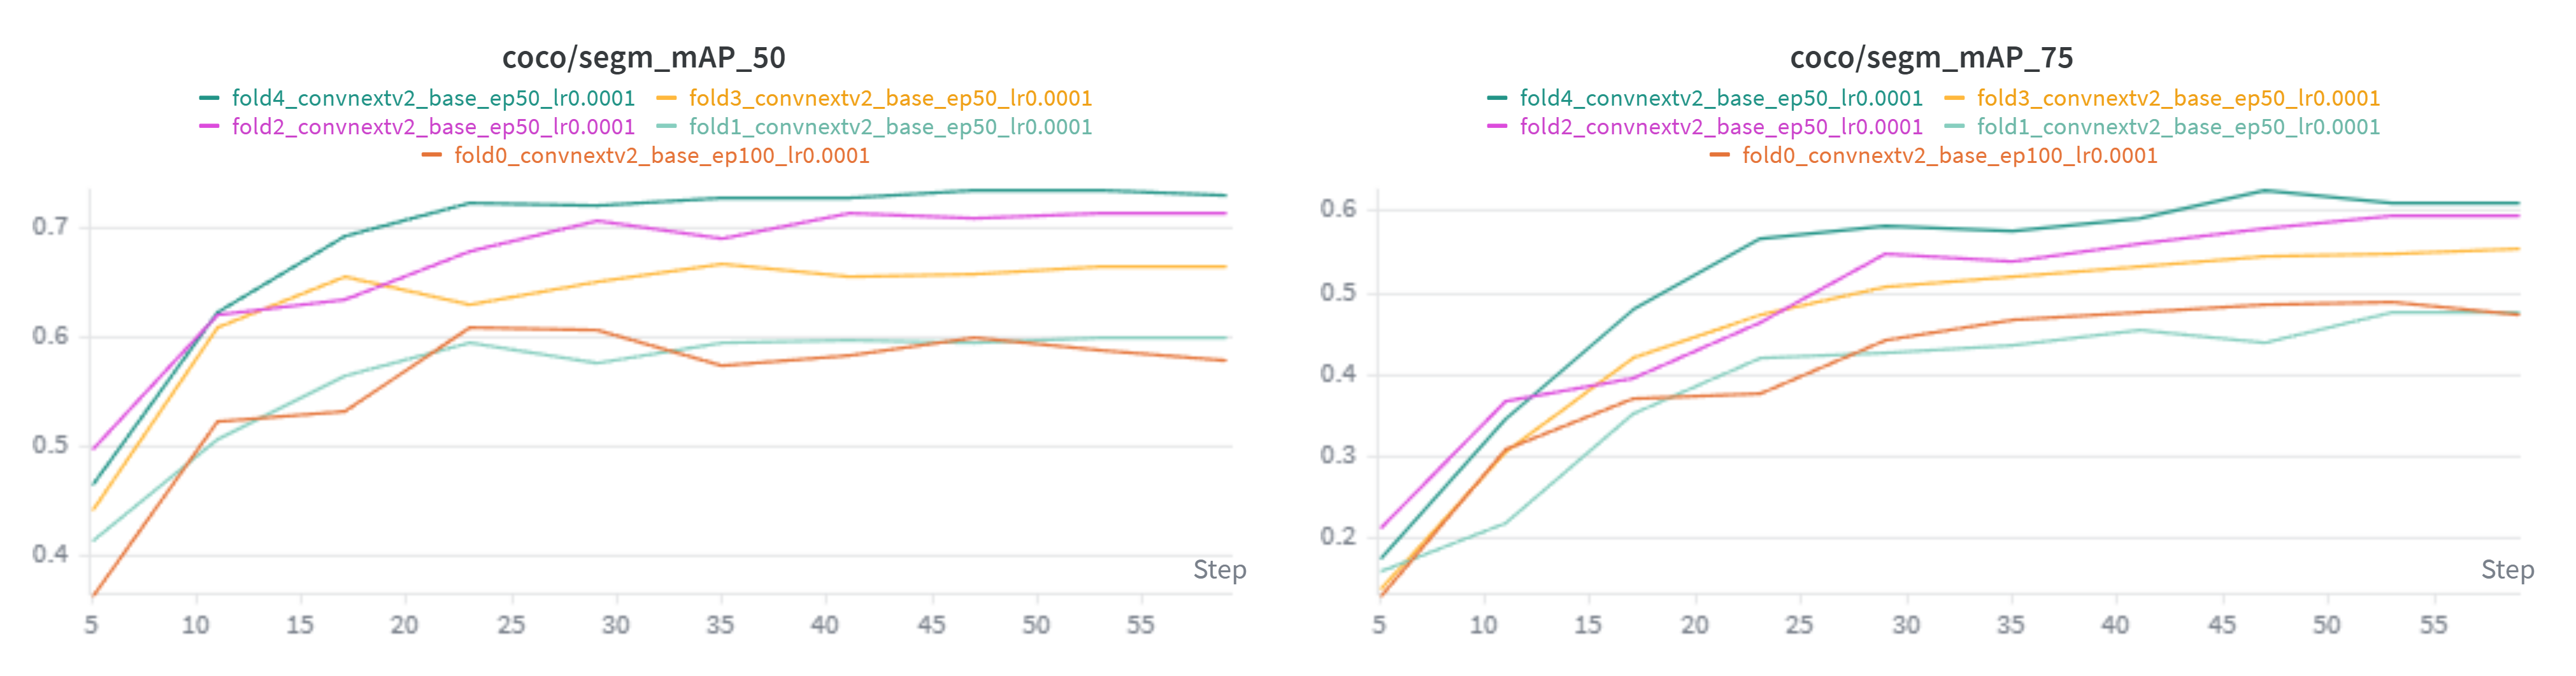
\includegraphics[width=0.95\linewidth]{figures/five_fold_validation_score.png}
\caption{Validation mAP across 5 folds. }
\label{fig:five_fold_validation_score}
\end{figure}

Figure \ref{fig:five_fold_validation_score} shows the validation mAP for each fold across epochs. Most folds achieve a peak validation mAP above 0.60, with Fold 2 and Fold 4 reaching approximately 0.70. Despite the large variance in validation mAP across folds, all folds yield a similar test mAP of approximately 0.56 to 0.58 on the test set. This discrepancy is likely attributable to the small validation set size, which may cause the difficulty level to vary considerably across folds.


\begin{figure}[H]
\centering
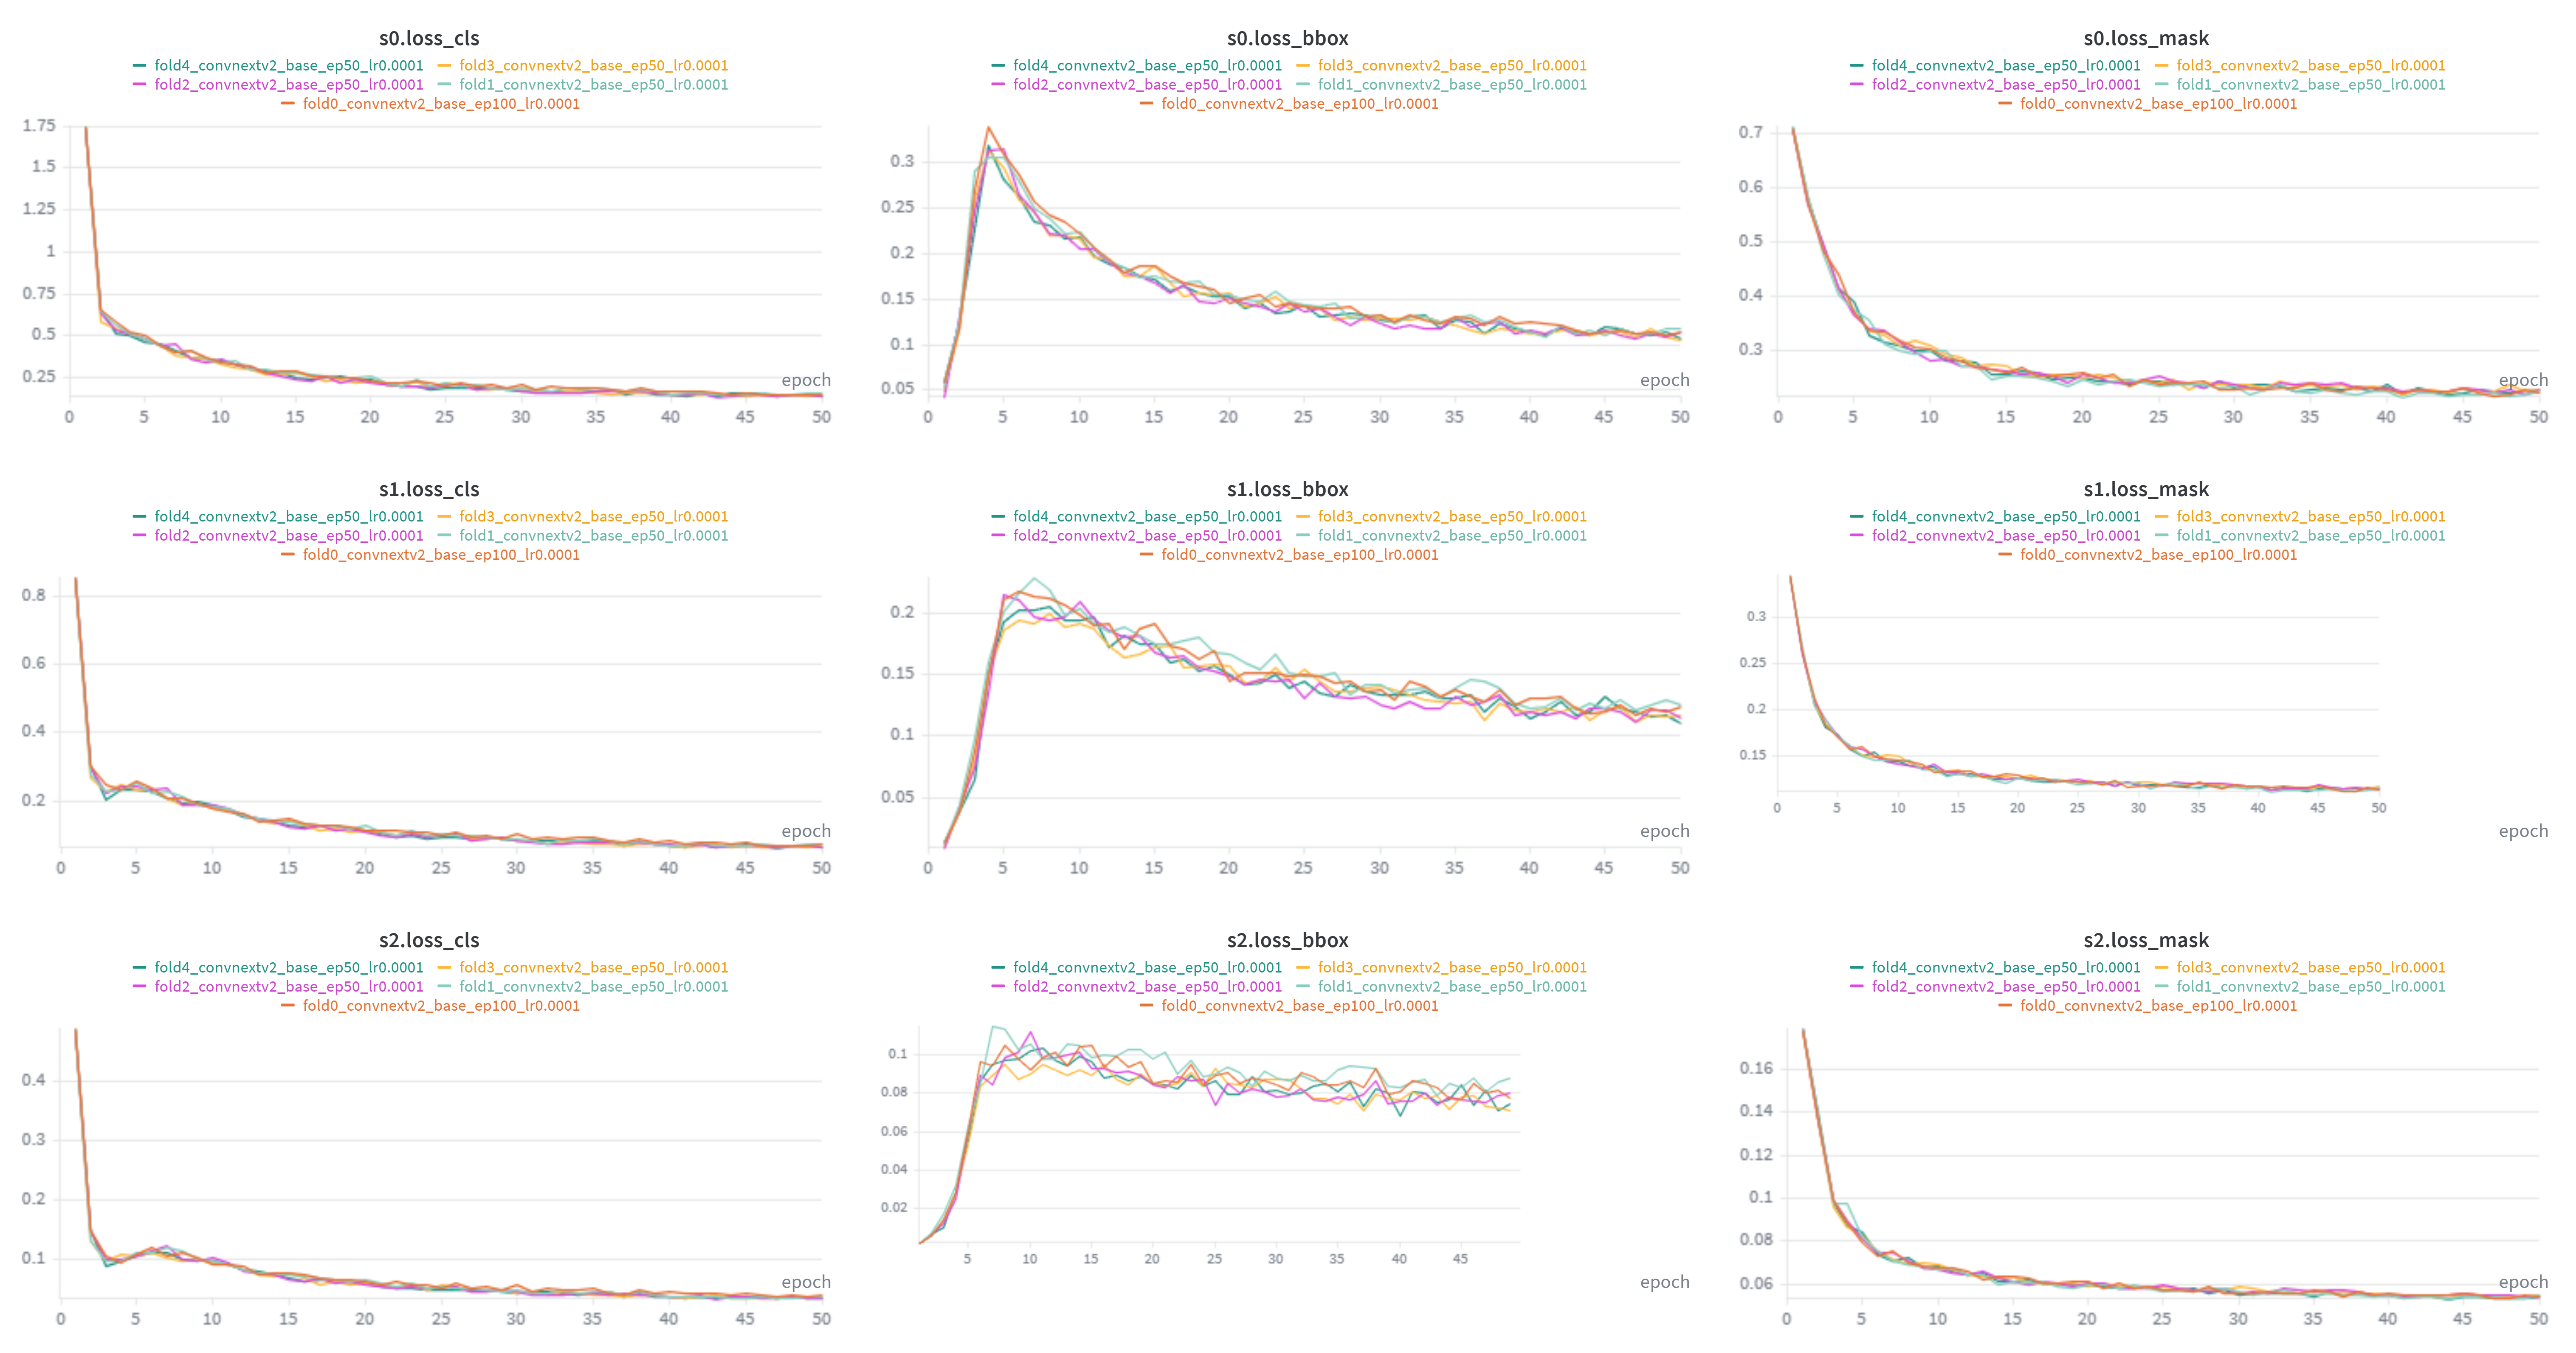
\includegraphics[width=0.95\linewidth]{figures/3stage_ROI_loss.png}
\caption{Cascade RoI head loss curves for the three stages, which contain classification, bbox regression, and mask loss. As shown in the figure, the loss decreases steadily across epochs for all three stages, indicating that the model is successfully learning to refine proposals and predict accurate masks. }
\label{fig:3stage_roi_loss}
\end{figure}


\begin{figure}[H]
\centering
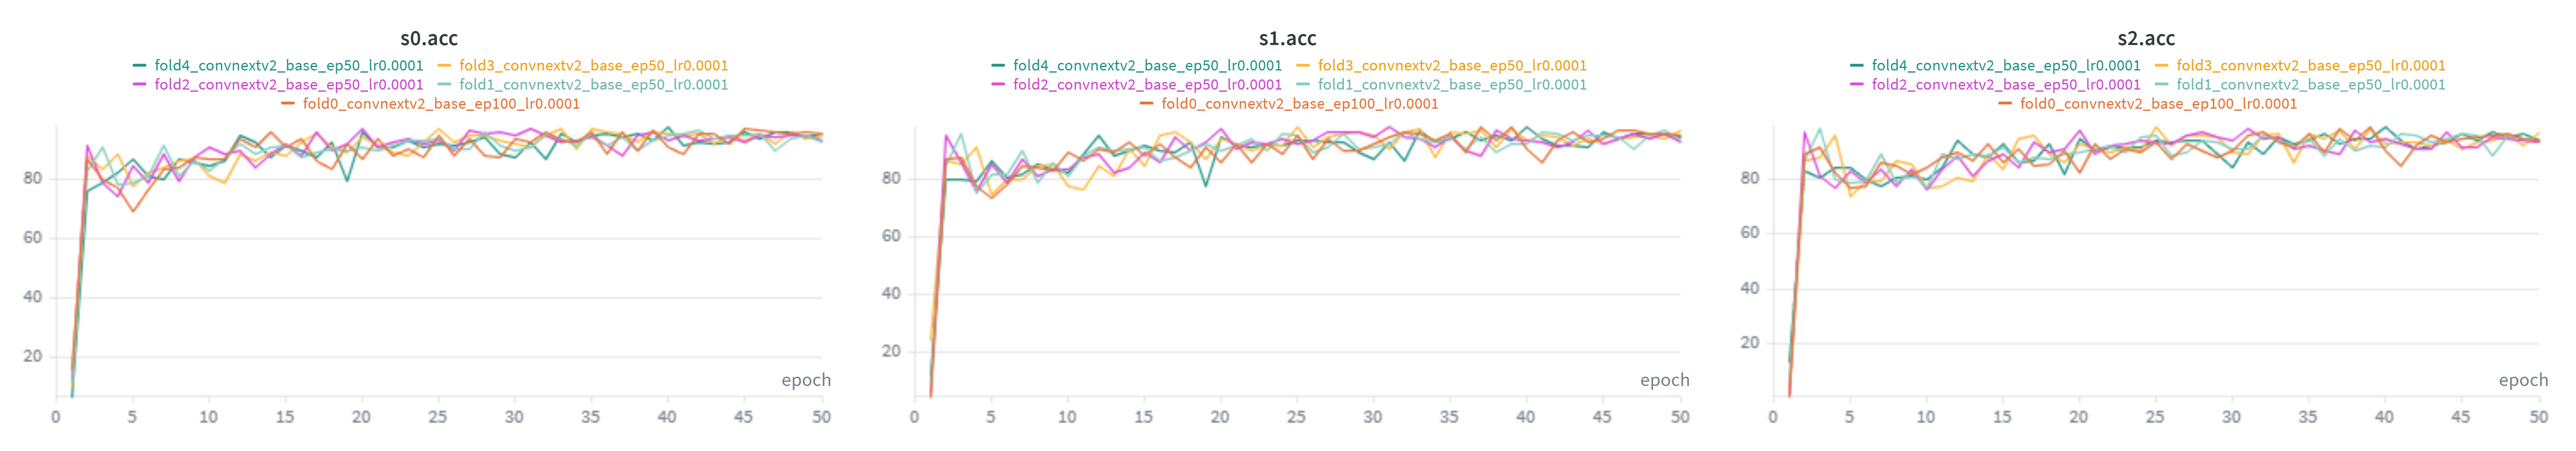
\includegraphics[width=0.95\linewidth]{figures/rol_head_acc.png}
\caption{The classification accuracy of the three cascade stages. The last stage (IoU=0.7) achieves the highest accuracy, which indicates that the cascade structure successfully refines the proposals to higher quality across stages. Let alone the slight difference, the accuracy reach around 0.95 for each stage, which indicates that each RoI head are capable of successfully classify the cell types on their own.}
\label{fig:rol_head_acc}
\end{figure}

\begin{figure}[H]
\centering
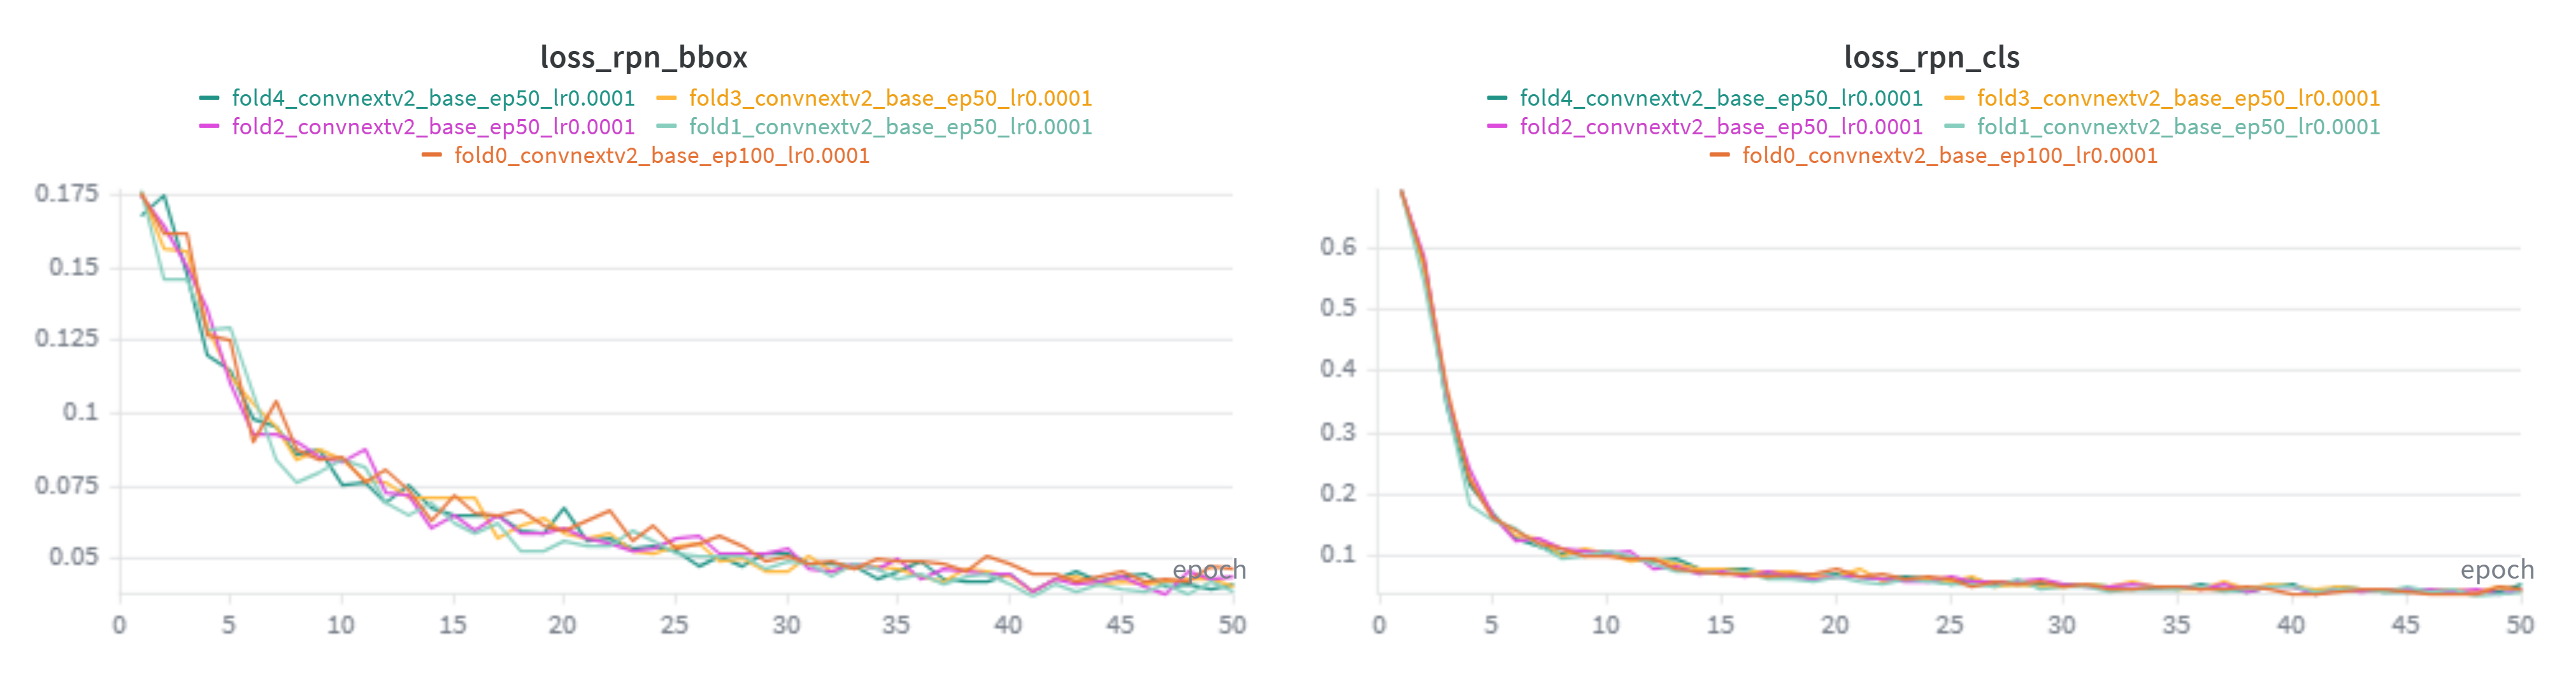
\includegraphics[width=0.95\linewidth]{figures/rpn_loss.png}
\caption{RPN loss curves for classification and regression. As shown in the figure, the loss decreases steadily across epochs, indicating that the RPN is successfully learning to generate high-quality proposals. }
\label{fig:rpn_loss}
\end{figure}

\begin{figure}[H]
\centering

\includegraphics[width=0.95\linewidth]{figures/test_score.png}
\caption{Final test score after TTA and WBF ensemble across all 5 fold models. The final mAP@50 is 0.6142, which empirically validating the effectiveness of our ensemble strategy. The performance gain demonstrates that TTA successfully enhances model robustness against orientation and scale variances, while the WBF mechanism effectively leverages the consensus across different folds to suppress noise and refine instance boundaries.}
\label{fig:test_score}
\end{figure}

\section{Additional Experiments}

\begin{figure}[H]
\centering
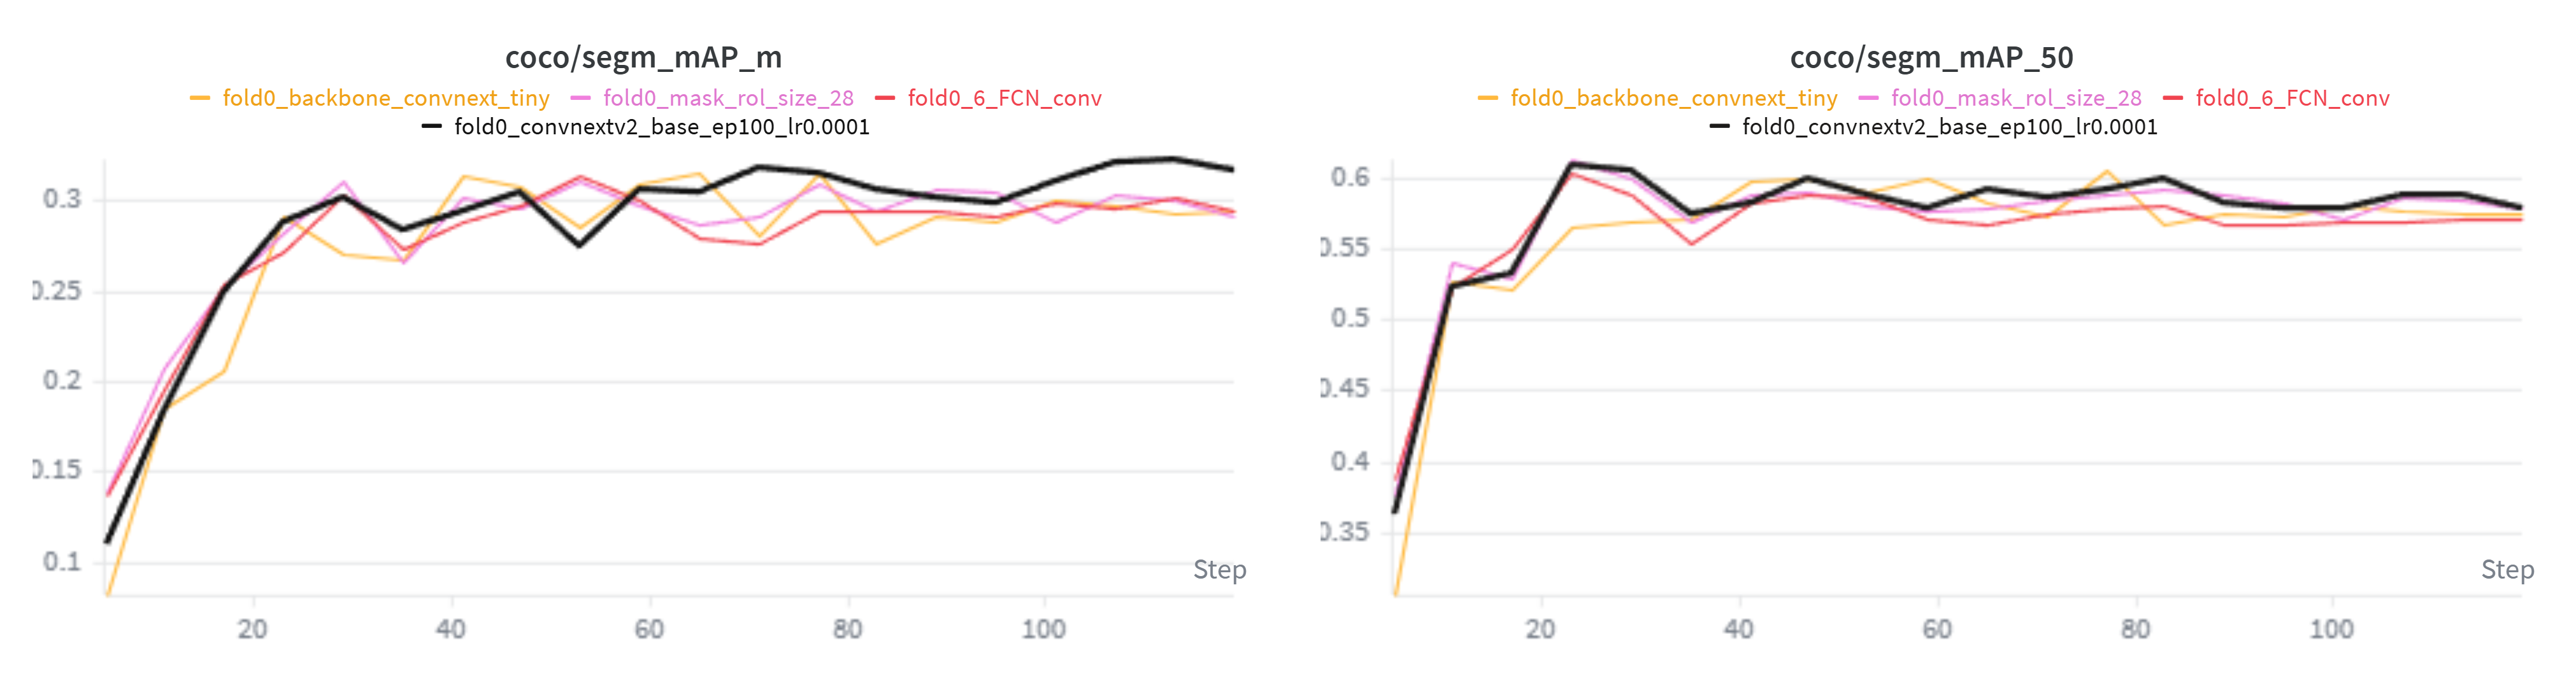
\includegraphics[width=0.95\linewidth]{figures/experiment_on_rol_mask_size_fcn_layer_backbone_tiny_convnext.png}
\caption{Ablation study on different architectural choices and hyperparameters.}
\label{fig:ablation_study_1}
\end{figure}

To evaluate the impact of different hyperparameters and architectural choices, we conducted three independent ablation experiments: (1) switching the backbone to \texttt{ConvNeXt-Tiny}, (2) increasing the \texttt{mask\_roi\_size} from 14 to 28, and (3) deepening the \texttt{FCNMaskHead} from 4 to 6 convolution layers. 

\begin{itemize}
    \item \textbf{Backbone Capacity (ConvNeXt-Tiny vs. Base):} Reducing the backbone to \texttt{ConvNeXt-Tiny} resulted in performance nearly identical to the \texttt{ConvNeXt-V2-Base} model. This suggests that for this specific cell segmentation task, the feature extraction capability of the "Tiny" variant is already sufficient, and the higher capacity of the "Base" model provides marginal gains, likely due to the limited diversity or size of the training samples.
    \item \textbf{Mask Resolution (RoI Size 14 vs. 28):} Increasing the \texttt{mask\_roi\_size} to 28 effectively boosts the spatial resolution of the mask branch, producing a $56 \times 56$ output compared to the default $28 \times 28$. However, this modification did not yield a significant increase in mAP. We attribute this to the potential noise in the ground truth masks; when the resolution is too high, the model may attempt to overfit to annotation irregularities rather than learning generalized cell morphologies.
    \item \textbf{Mask Head Depth (FCN Layers 4 vs. 6):} Deepening the \texttt{FCNMaskHead} was intended to enhance the non-linear representational power of the mask branch. Contrary to expectations, the 6-layer configuration exhibited signs of overfitting toward the end of the training epochs. The increased parameter count in the mask head likely caused the model to memorize specific training instances instead of improving its boundary refinement capabilities.
\end{itemize}

\textbf{Conclusion on Overfitting:} These results indicate that the baseline configuration—consisting of \texttt{ConvNeXt-V2-Base} with a 4-layer mask head and a \texttt{mask\_roi\_size} of 14—sits at an optimal balance point between model complexity and data scale. Further increasing the model's depth or resolution leads to diminishing returns and eventual overfitting, as the model exhausts the meaningful information available in the training signal.


\begin{figure}[H]
\centering
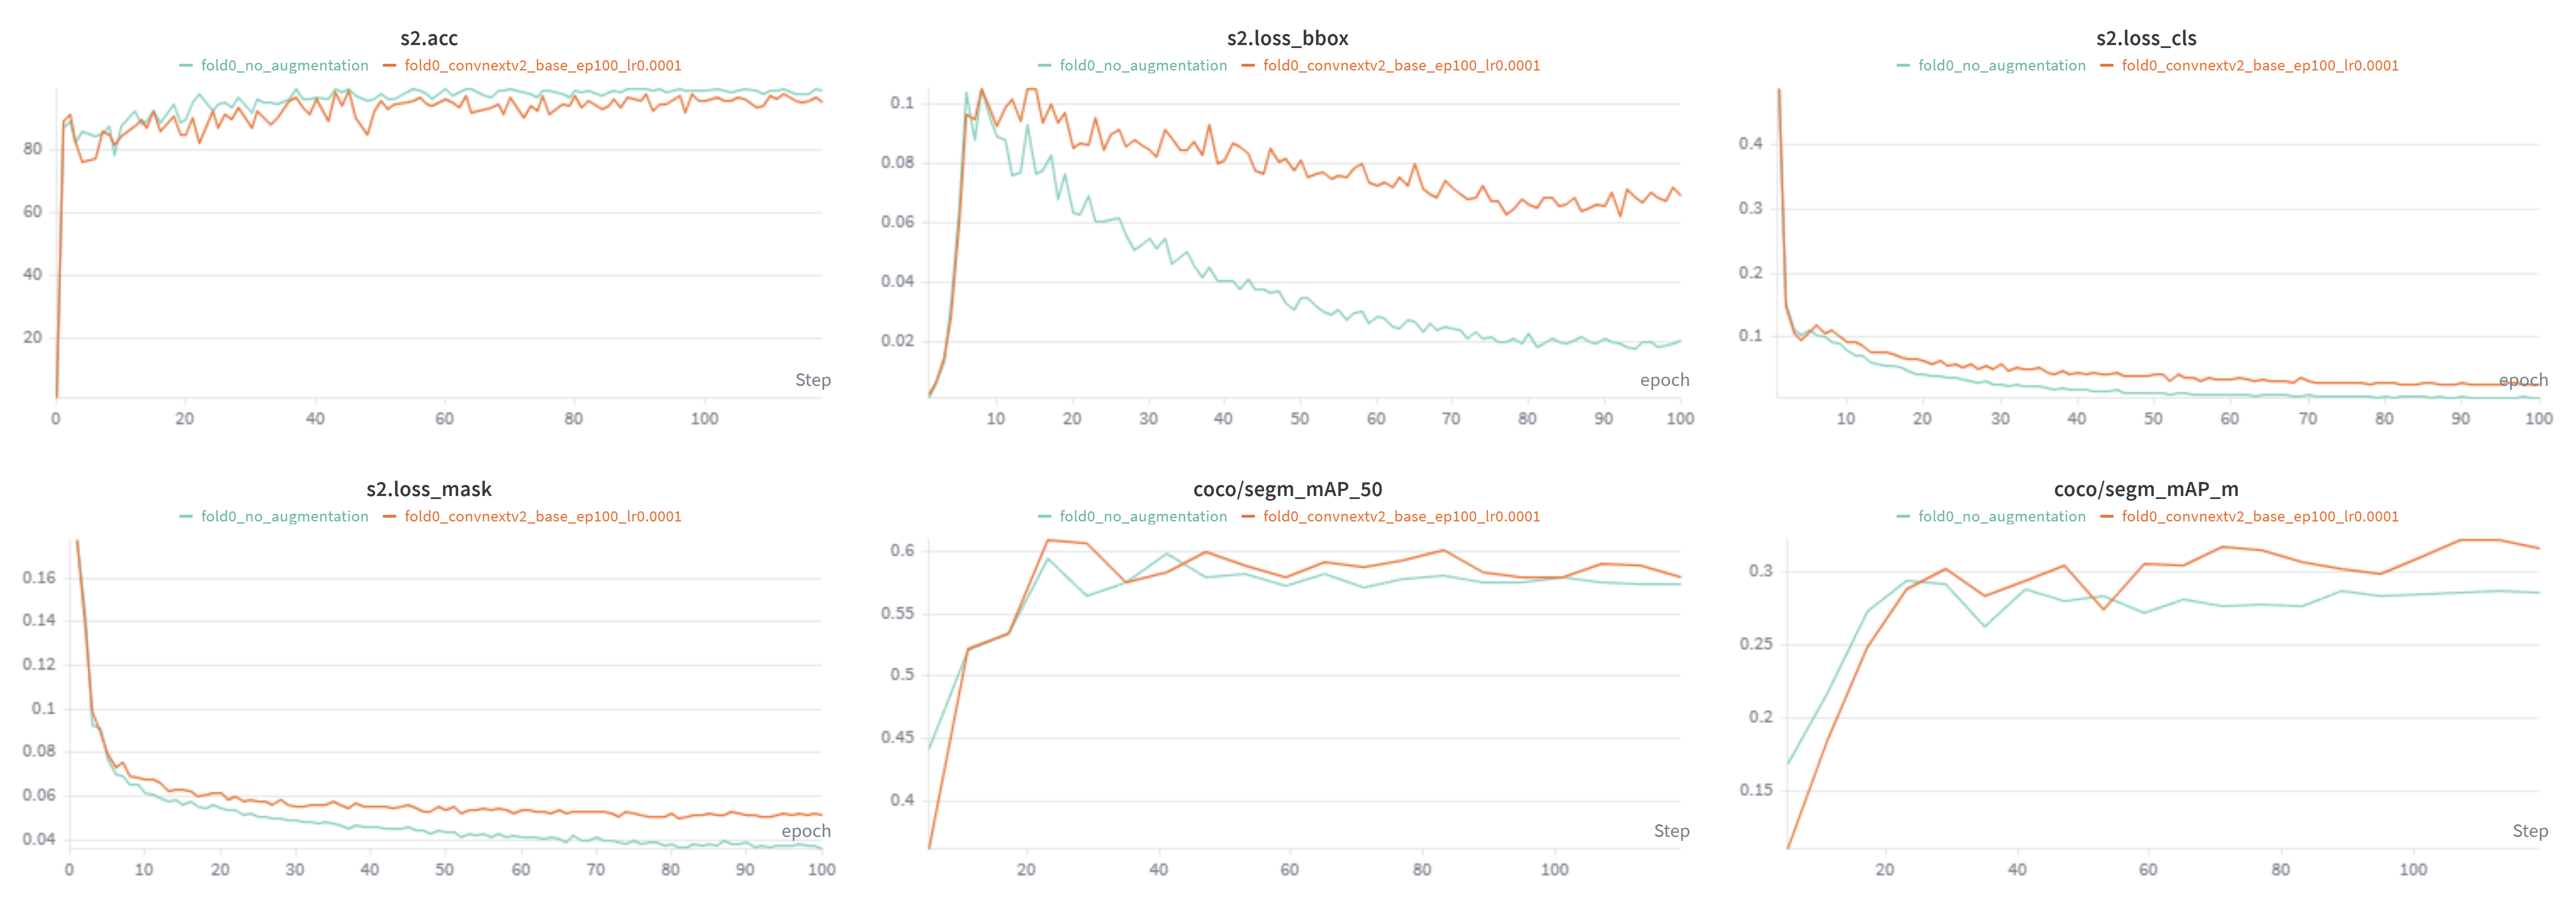
\includegraphics[width=0.95\linewidth]{figures/no_aug.png}
\caption{Ablation study on the impact of data augmentation.}
\label{fig:ablation_study_augmentation}
\end{figure}


To quantify the contribution of our data augmentation pipeline, we conducted a controlled experiment by training a model with all augmentations removed (shown in figure \ref{fig:ablation_study_augmentation}), serving as a baseline for comparison. The objective was to isolate the effect of geometric and color transformations on the model's ability to learn generalized features. Theoretically, a model trained without augmentation should minimize training loss more rapidly due to the simplified data distribution; however, it is expected to suffer from poor generalization on unseen validation data.

The experimental results provide the following insights:

\begin{itemize}
    \item \textbf{Training Convergence:} The model without augmentation (represented by the blue line in \texttt{no\_aug.jpg}) exhibits a significantly faster and deeper decline in training losses, particularly in \texttt{s2.loss\_bbox} and \texttt{s2.loss\_mask}. This indicates that the model is highly efficient at "memorizing" the raw pixel distributions of the specific training samples.
    \item \textbf{Generalization Gap:} Despite the superior training metrics, the validation performance of the "no-augmentation" model is inferior to the augmented baseline (represented by the orange line). As shown in the \texttt{coco/segm\_mAP\_50} and \texttt{coco/segm\_mAP\_m} plots, the augmented model consistently achieves higher mAP scores in the later stages of training.
    \item \textbf{Overfitting Implications:} The divergence between the training loss and validation mAP in the non-augmented model suggests a classic case of overfitting. The higher training loss observed in our proposed \texttt{ConvNeXt-V2-Base} configuration is an indicator of effective regularization, where the model is forced to learn transformation-invariant features rather than specific image instances.
\end{itemize}

In conclusion, while removing augmentations accelerates convergence, it results in a lower performance ceiling. These findings empirically validate that our augmentation strategy is essential for bridging the gap between training and real-world inference in complex cell segmentation tasks.


\begin{figure}[H]
\centering
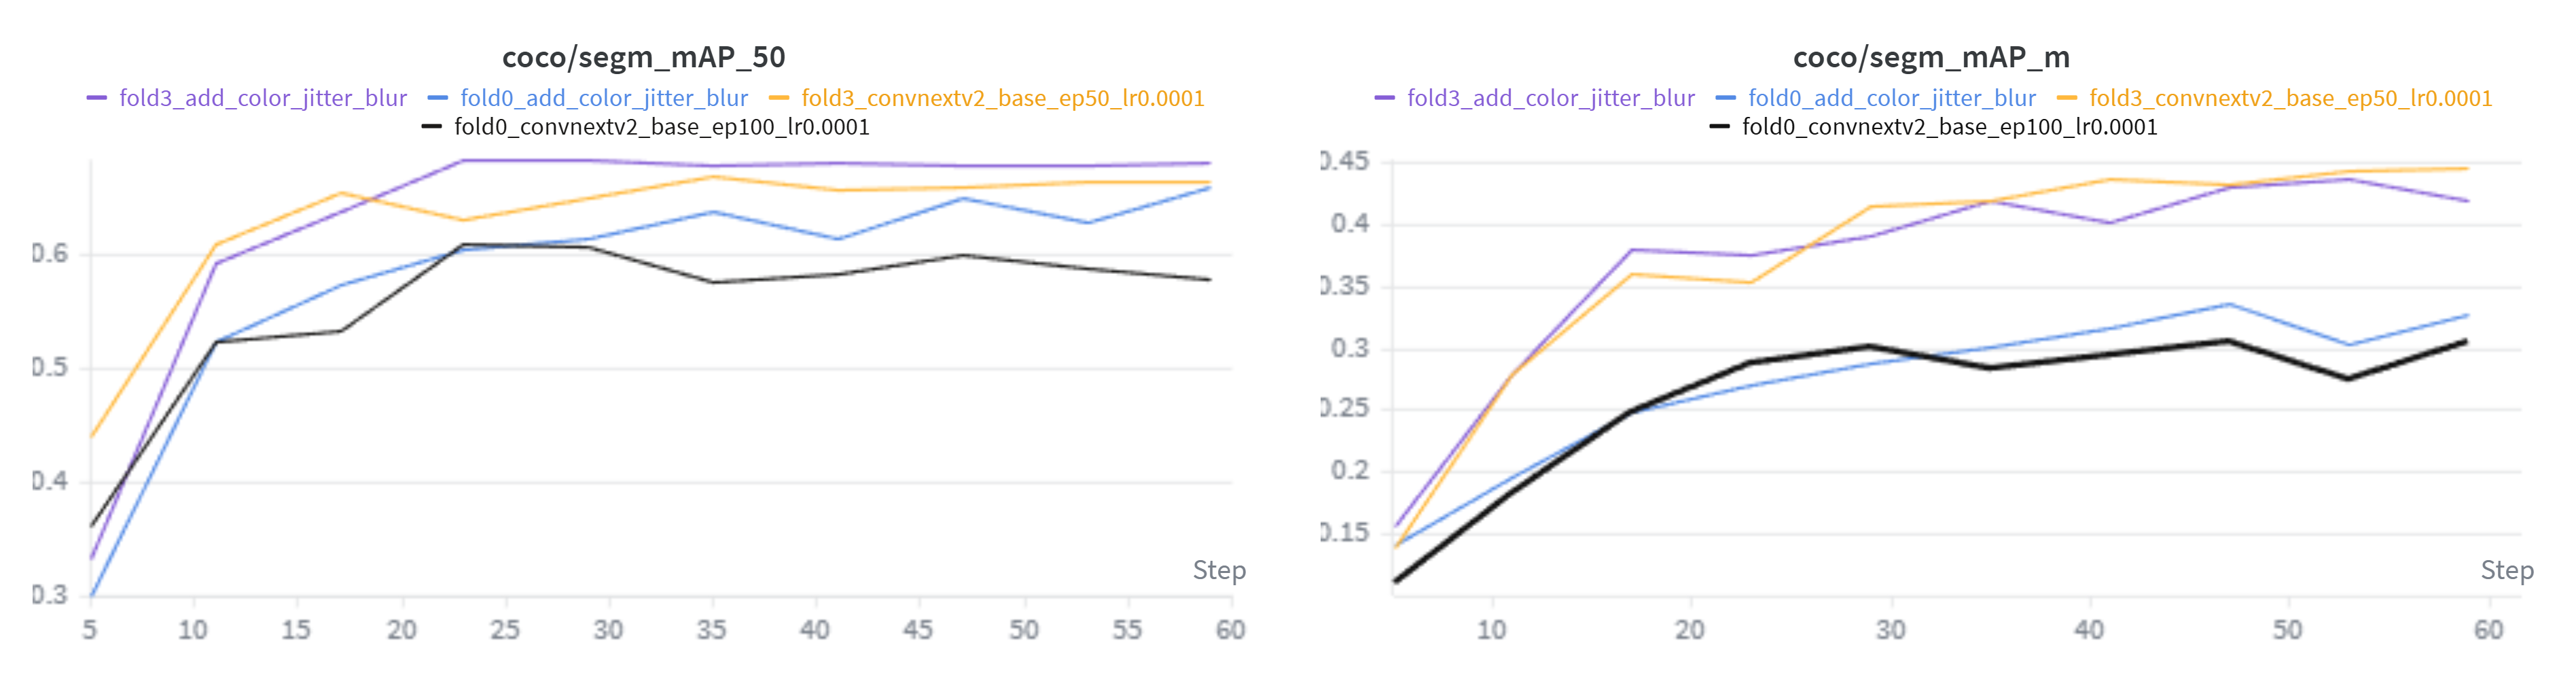
\includegraphics[width=0.95\linewidth]{figures/add_color_jitter_blur.png}
\caption{Ablation study on the impact of adding color jitter and Gaussian blur to the augmentation pipeline.}
\label{fig:ablation_study_jitter_blur}
\end{figure}

To further improve the robustness of the model, we conducted an experiment by adding \textbf{Color Jitter} and \textbf{Gaussian Blur} to the existing augmentation pipeline. The motivation was to simulate variations in lighting, staining intensity, and sensor noise common in biological imaging. While this strategy successfully enhanced the validation performance of certain folds, it failed to yield a corresponding improvement on the final test bench.

As shown in the validation curves (Figure \ref{fig:ablation_study_jitter_blur}), the introduction of these augmentations provided a noticeable boost to the \texttt{mAP@50} and \texttt{mAP\_m} for \textbf{Fold 0} and \textbf{Fold 3}, which had previously exhibited lower performance. However, the stagnant test score suggests several critical implications:

\begin{itemize}
    \item \textbf{Distribution Mismatch and Domain Shift:} The performance gain on specific folds indicates that these subsets likely contained images with lighting or clarity issues that the added augmentations helped regularize. However, the test set may be relatively "clean" or contain a different distribution of artifacts. Consequently, the model learned to handle synthetic noise that does not exist in the actual test data, leading to a "phantom" improvement in local validation.
    \item \textbf{Overfitting to Synthetic Noise Patterns:} By training with Gaussian blur and color jitter, the model may have focused on learning the specific mathematical kernels and pixel-level perturbations provided by the augmentation libraries. This can lead the model to prioritize "denoising" or "re-coloring" rather than extracting the underlying morphological features of the cells, which are the true indicators of instance boundaries.
    \item \textbf{Saturation of Feature Discriminability:} Given the high capacity of the \texttt{ConvNeXt-V2-Base} backbone, the model may have already reached its peak discriminative power for the given dataset. Adding further pixel-level noise might only shift the internal feature distributions without providing additional structural information necessary to improve the final mAP on the public leaderboard.
\end{itemize}

In summary, while adding color and noise augmentations is a common practice to boost robustness, its effectiveness is highly dependent on the alignment between synthetic transformations and the actual variance in the hidden test distribution. In this case, the results suggest that the baseline geometric augmentations (e.g., rotation, flipping) were already sufficient to capture the essential invariance required for the task.

\printbibliography % to print the bibliography
\end{document}
